\begin{frame}{Acoustic Species}
\end{frame}


% introduction on bird species conservation, and how aucoustic monitoring is done
\begin{frame}{Passive Acouistic Monitoring}
    \centering
    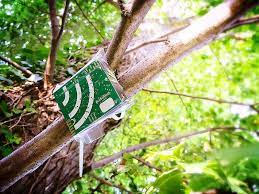
\includegraphics[height=0.7\textheight,width=0.7\textwidth,keepaspectratio]{pam.jpeg}
\end{frame}


% Explanation on how deep learning can be applied to audio data through spectrograms (seems easy!)
\begin{frame}{Spectrogram}
    \centering
    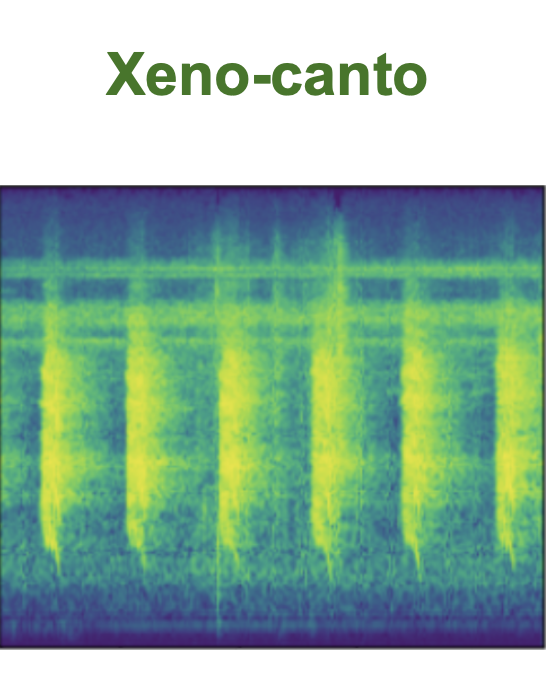
\includegraphics[height=0.7\textheight,width=0.7\textwidth,keepaspectratio]{xeno.png}
\end{frame}


% (plot twist) the soundscape data is drastically different from our training data
\begin{frame}{}
    \begin{columns}
        \begin{column}{0.5\textwidth}
            \centering
            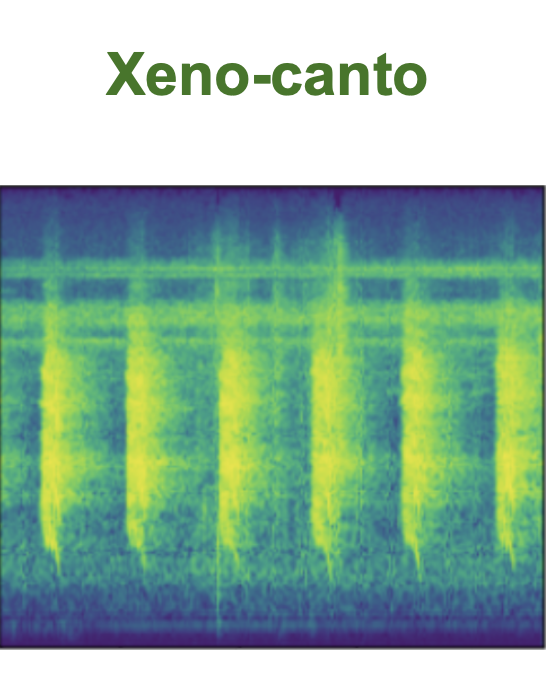
\includegraphics[height=0.7\textheight,width=0.7\textwidth,keepaspectratio]{xeno.png}
        \end{column}
        \begin{column}{0.5\textwidth}
            \centering
            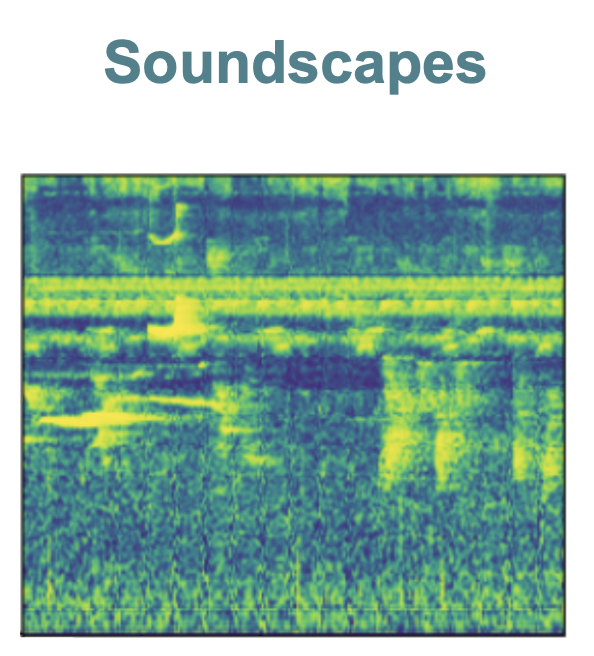
\includegraphics[height=0.7\textheight,width=0.7\textwidth,keepaspectratio]{soundscape.png}
        \end{column}
    \end{columns}
\end{frame}



% Actions taken to improve model performance on soundscape data
\begin{frame}{How do we improve?}
    \begin{itemize}
        \item Data Augmentation
        \item Model Ensembling
        \item Modified CNN with updated kernel for audio
    \end{itemize}    
\end{frame}

%
% Leave this part for surangana, GUI

% ending slide, I will talk about the labelling party and how it will guide our summer research
\begin{frame}{So what now?}
\end{frame}
